
\section{Laplace-Transformation \skript{74}}
	$$\boxed{f(t) \; \laplace \; F(s)=\int\limits_0^\infty f(t)e^{-st}dt} \qquad \boxed{ s=\sigma+j\omega}$$\\
	\begin{itemize}
		\item Originalfunktion $ f(t) \; \laplace \; F(s)$ Bildfunktion
		\item Definitionsbereich nur für kausale Systeme $t\geq 0$
		%\item Integrierbar über das Intervall $(0,\infty)$\\
		\item  Wachstum kleiner als der von einer Exponentialfunktion
		\item  Gegen"uber $j\omega$ bei der Fourier-Transformation ist bei der
			Laplace-Transformation $s$ verallgemeinert zu $s=\sigma + j\omega$. Das
			bedeutet, dass die Fourier-Transformierte $F(j\omega)$ durch die
			Laplace-Transformation $F(s)$ ausgedr\"uckt werden kann.
		\item  mit 
		$\begin{cases} 
		\sigma = 0 & \rightarrow \text{Amplitude bleibt konstant} \\ 
		\sigma > 0 & \rightarrow \text{explodiert die Amplitude f\"ur } 0 < t \rightarrow \infty \\
		\sigma < 0 & \rightarrow \text{klingt die Amplidute für } 0 < t \rightarrow \infty \text{ auf $0$ ab} \
		 \end{cases} $ \\   
	\end{itemize}



	
 	\subsection{Eigenschaften der Laplace-Transformation \skript{74}}
 	
	  \renewcommand{\arraystretch}{2}
		\begin{tabular}{|p{2.5cm}|p{3cm}|p{2.5cm}p{10cm}|}
			\hline
				\multicolumn{3}{|l}{Linearität}   &  $\alpha\cdot f(t) + \beta\cdot g(t) \; \laplace \; \alpha\cdot F(s) + \beta\cdot G(s) \qquad\qquad (\alpha, \beta \in\mathbb{C})$ \\ 
			\hline
				\multicolumn{3}{|l}{"Ahnlichkeit / Streckung im Zeitbereich}   &  $f(\alpha t) \; \laplace \; \frac{1}{\alpha}F \left (\frac{s}{\alpha} \right ) \hspace{4cm} (0 <\alpha, \alpha \in\mathbb{R})$ \\
			\hline
			\hline
				\multirow{3}{*}{Verschiebung} & \multirow{2}{*}{Zeitbereich} & nach links &  $\sigma(t+a) \cdot f(t + a) \; \laplace \; e^{as} \cdot [F(s) - \int\limits_0^{a} f(t) \cdot e^{-st} dt]$	 \\ \cline{3-4} 
				&  & nach rechts  & $\sigma(t-a) \cdot f(t - a) \; \laplace \; F(s) \cdot e^{-as}$ \\ \cline{2-4}
				& \multicolumn{2}{l}{Frequenzbereich (Dämpfungssatz)} & $f(t) \cdot e^{\pm\alpha t} \; \laplace \; F(s\mp\alpha)$\\ 
			\hline
			\hline
				\multirow{2}{*}{Faltung} & \multicolumn{2}{l}{Zeitbereich} & $f(t) \ast g(t) = \int\limits_{0}^{t} f(\tau) \cdot g(t-\tau) \; d\tau \; \laplace \; F(s)
				\cdot G(s)$ \\ \cline{2-4} 
				& \multicolumn{2}{l}{Frequenzbereich} &  $f(t) \cdot g(t) \; \laplace \; \frac{1}{2\pi j}\int\limits_{c-j\infty}^{c+j\infty}
				F(\xi) \cdot G(s-\xi) \; d\xi$\\ 
			\hline
			\hline
				\multirow{4}{*}{Ableitung} & \multirow{3}{*}{Zeitbereich} & 1te & 	$\frac{\partial f(t)}{\partial t} \; \laplace \; sF(s)-f(0^+)$ \\ \cline{3-4}
				&  & 2te  &  $\frac{\partial^2 f(t)}{\partial t^2} \; \laplace \; s^2F(s)		-sf(0^+) -f'(0^+)$\\ \cline{3-4}
				&  & nte  &  $\frac{\partial^n f(t)}{\partial t^n} \; \laplace \; s^nF(s)
				-s^{n-1}f(0^+)-s^{n-2}\frac{\partial f(0^+)}{\partial t}-\ldots
				-s^0\frac{\partial^{n-1} f(0^+)}{\partial t^{n-1}}$\\ \cline{2-4} 
				& \multicolumn{2}{l}{Frequenzbereich} & $(-t)^n \cdot f(t) \; \laplace \;  \frac{\partial^n F(s)}{\partial s^n} \qquad \hspace{2cm} (n \in \mathbb{N}_0)$\\
			\hline
			\hline
				\multicolumn{3}{|l}{Integration im Originalbereich (Sprungantwort)}   &  $\int\limits_0^t f(u) \; du \; \laplace \; \frac{1}{s}\cdot F(s)$ \\
			\hline
			\hline
				\multicolumn{3}{|l}{Multiplikation mit $t$}  &
				$t\cdot f(t)  \; \laplace \; \frac{-d F(s)}{d s}$\\
			\hline
			\hline
				\multicolumn{3}{|l}{Anfangswert}   &  	 			$\lim\limits_{t\rightarrow 0^+} f(t) = \lim\limits_{s\rightarrow \infty} sF(s),\text{~wenn
				}  \lim\limits_{t\rightarrow 0} f(t)\text{~existiert}.$\\
			\hline
				\multicolumn{3}{|l}{Endwert}   & 	 			$\lim\limits_{t\rightarrow \infty} f(t) = \lim\limits_{s\rightarrow 0} sF(s),\text{~wenn
				}  \lim\limits_{t\rightarrow \infty} f(t)\text{~existiert}.$ \\ 
			\hline
		\end{tabular}
	\renewcommand{\arraystretch}{\arraystretchOriginal}
		
		
		
		
		
		
	
	\subsection{Laplace-Tabelle \bronstein{1127-1132}}
	\renewcommand{\arraystretch}{2}
	\hrule
	\begin{minipage}{9cm}
		\begin{center}
			\begin{tabular}{p{4cm}p{0.75cm}p{3cm}}
				$\sigma \left( t \right)$ & $\; \laplace \;$ & $\dfrac{1}{s}$ \\
				
				$\sigma \left( t \right) \cdot t$ & $\; \laplace \;$ & $\dfrac{1}{s^2}$\\
				
				$\sigma \left( t \right) \cdot t^2$ & $\; \laplace \;$ & $\dfrac{2}{s^3}$\\
				
				$\sigma \left( t \right) \cdot t^n$ & $\; \laplace \;$ & $\dfrac{n!}{s^{n+1}}$\\
				
				$\sigma \left( t \right) \cdot e^{\alpha t}$ & $\; \laplace \;$ &
				$\dfrac{1}{s-\alpha}$\\
				
				$\sigma \left( t \right) \cdot t \cdot e^{\alpha t}$ & $\; \laplace \;$ & $\dfrac{1}{( s - \alpha )^2}$\\
				
				$\sigma \left( t \right)\cdot t^2 \cdot e^{\alpha t}$ &
				$\; \laplace \;$ & $\dfrac{2}{{( s - \alpha )}^3}$\\
				
				$\sigma \left( t \right)\cdot t^n \cdot e^{ \alpha t}$ &
				$\; \laplace \;$ & $\dfrac{n!}{(s-\alpha)^{n+1}}$\\
				
				$\sigma \left( t \right)\cdot \dfrac { 1 - e ^ { - \alpha t } } { \alpha }$ & $\; \laplace \;$ & $\dfrac { 1 } { s ( s + \alpha ) }$\\
				
				$\sigma \left( t \right)\cdot \dfrac {e ^ { - \alpha t }+\alpha t -1 } { \alpha^2 }$ & $\; \laplace \;$ & $\dfrac { 1 } { s^2 ( s + \alpha ) }$\\
				
				$\sigma \left( t \right)\cdot \dfrac {1- e ^ { - \alpha t } - \alpha t e ^ {- \alpha t }}{ \alpha ^2 }$ & $\; \laplace \;$ & $\dfrac { 1 } { s ( s + \alpha )^2 }$\\
					
			\end{tabular}
		\end{center}
	\end{minipage}
\vline
\begin{minipage}{9cm}
\begin{center}
	\begin{tabular}{p{5cm}p{0.75cm}p{3cm}}
	
		$\delta \left( t \right)$ & $\; \laplace \;$ & $1\left( s \right)$ \\
		
		$\delta \left( t - \alpha \right)$ & $\; \laplace \;$ & $e^{- \alpha s}$\\
		
		$\sigma\left( t - \alpha \right)$ & $\; \laplace \;$ & $ \dfrac{1}{s} \cdot e^{- \alpha s}$\\
		
		$\sigma \left( t \right) \cdot \sin \left(\omega t \right)$ & $\; \laplace \;$ &
		$\dfrac{\omega}{s^2 + {\omega^2}}$\\
		
		$\sigma \left( t \right) \cdot \cos \left( \omega t \right)$ & $\; \laplace \;$ &
		$\dfrac{s}{ s^2 + \omega^2}$\\
		
		$\sigma \left( t \right) \cdot  e^{ \alpha t} \cdot \sin \left(\omega t \right)$ & $\; \laplace \;$ 
		& 	$\dfrac{\omega}{(s-\alpha)^2 + {\omega^2}}$\\
		$\sigma \left( t \right) \cdot e^{ \alpha t} \cdot \cos \left( \omega t \right) $ & $\; \laplace \;$ &
		$\dfrac{s-\alpha}{(s-\alpha)^2 + \omega^2}$\\
		
		$\sigma \left( t \right)\cdot t \cdot \dfrac{\sin \left( \alpha t \right)} { 2 \alpha }$ & $\; \laplace \;$ & $\dfrac{s}{ \left(s^ {2}+ \alpha ^{2} \right)^{2}}$ \\
		
		$\sigma \left( t \right)\cdot \dfrac { e ^ { - \alpha t } - e ^ { - \beta t } } { \beta - \alpha }$ & $\; \laplace \;$ & $\dfrac { 1 } { ( s + \alpha ) ( s + \beta ) }$\\
		
		$\sigma \left( t \right)\cdot \dfrac {(\alpha - \beta) +\beta e ^ { - \alpha t } - \alpha e ^ { - \beta t } } { \alpha \beta (\alpha - \beta) }$ & $\; \laplace \;$ & $\dfrac { 1 } {s ( s + \alpha ) ( s + \beta ) }$\\
		
		$\sigma \left( t \right)\cdot \dfrac { e ^ { - \beta t } ( \alpha \cos ( \alpha t ) - \beta \sin ( \alpha t ) ) } { \alpha }$& $\; \laplace \;$ & $\dfrac { s } { ( s + \beta ) ^ { 2 } + \alpha ^ { 2 } }$\\
		
		 
		
		
	\end{tabular}
\end{center}
\end{minipage}


\newpage
\renewcommand{\arraystretch}{\arraystretchOriginal}		
	\subsection{Rücktransformation \skript{85}}
		\subsubsection{Vorgehen}
			\begin{enumerate}
				\item Kürzen oder vereinfachen
				\item Partialbruchzerlegung falls nötig 
				\item Rücktransformation mittels Laplace-Tabelle
				\item $h(t)\hspace{0.2cm}\underline{nicht} < 0$
			\end{enumerate}
			
		\subsubsection{Residuensatz}
			\textbf{Beispiel:}\\[2mm]
			$F(s) = \dfrac{1}{(s+\alpha)(s+\beta)}, \qquad (0 < \alpha,\beta \in \mathbf{R}, \alpha \neq \beta)$\\[2mm]
			$f(t) = \frac{1}{2\pi j} \int\limits_{-j\infty}^{j\infty} F(s)e^{st} ds = \sum\limits_{i=1}^k Res(F(s_k)e^{s_kt})$\\[2mm]
			$=\lim_{s \to -\alpha} ((s+\alpha)F(s)e^{st}) + \lim_{s \to -\beta}((s+\beta)F(s)e^{st})$\\[2mm]
			$=\dfrac{e^{-\alpha t}}{\beta - \alpha} + \dfrac{e^{-\beta t}}{\alpha - \beta} = \dfrac{e^{-\alpha t}-e^{-\beta t}}{\beta - \alpha}$
			

	
	\subsection{Lösung linearer Differentialgleichungen \skript{88-105}}
			
			\begin{minipage}{12cm}

				\renewcommand{\arraystretch}{2}
					\begin{tabular}{| l | l |}		%TODO Tabelle, Paragraph für schönere Darstellung
						\hline
							Übertragungsfunktion & $G(s) = \dfrac{1}{p(s)}$\\
							& $g(t) \; \laplace \; G(s)$ \\
						\hline
							Frequenzgang \& \\ Übertragungsfunktion  & $H(\omega) = \dfrac{1}{p(j\omega)} = G(j\omega) $ \\
						\hline
							Impulsantwort & $y_{\delta}(t) = y_{\sigma}'(t) = g(t) \; \laplace \; G(s) = \dfrac{1}{p(s)}=Y_{\delta}(s)$\\
						\hline
							Sprungwantwort & $y_{\sigma}(t)=\int\limits_0^t g(u) \; du \; \laplace \; \dfrac{G(s)}{s} = \dfrac{1}{s \cdot p(s)} = Y_{\sigma}(s)$\\
						\hline
							Eigenschwingung & $Y(s) = \dfrac{h(s)}{p(s)} \quad \iff \quad p(s) \cdot Y(s)-h(s) = 0$ \\
						\hline
							äussere Erregung & $ Y(s) = F(s) \cdot \dfrac{1}{p(s)}$ \\
						\hline
							stationärer Zustand & = ungedämpfte Eigenschwingung\\
						\hline
						\hline
							Satz von Durhamel & $y(t) = y_{\sigma}'(t) * f(t)$\\
						\hline
					\end{tabular}
				\renewcommand{\arraystretch}{\arraystretchOriginal}\\
			
			\end{minipage}
			\begin{minipage}[b]{8cm}
				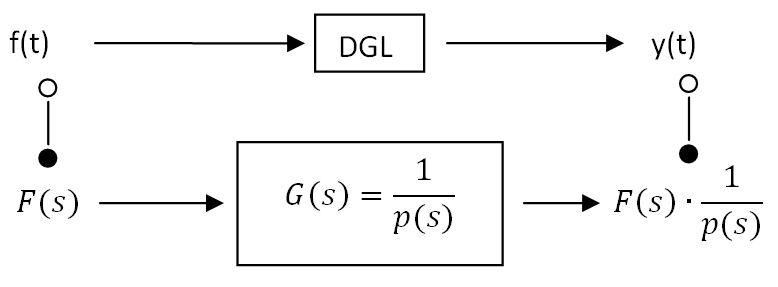
\includegraphics[width=8cm]{./bilder/diffgleichungen2.png} \\[7mm]

					\hspace{3cm}\begin{minipage}{4cm}
						$
						\begin{aligned}
							y(t) \; &\laplace \; Y(s) = F(s) \cdot \dfrac{1}{p(s)}\\
							g(t) \; &\laplace \; G(s) \\
						\end{aligned}
						$
					\end{minipage}	
			\end{minipage}

		

				
		
	\subsection{Eigenschwingung \skript{95}}
		\begin{minipage}{12cm}
			Spezielle Anfangswerte bei einem System ohne äussere Einflüsse:\\
			$y(0) = 0, y'(0) = 0, \dots , y^{(n-2)} = 0, y^{(n-1)} = 1$\\
			in diesem Fall wird $h(s) = 1$\\
		\end{minipage}
		\begin{minipage}{6cm}
			\begin{math}
				\begin{aligned}
					y(t) \; &\laplace \; Y(s)\\
					y'(t) \; &\laplace \; sY(s) - y_0\\
					y''(t)\; &\laplace \; s^2Y(s) - sy_0 - y'_0\\ 
					y'''(t)\; &\laplace \; s^3Y(s) - s^2y_0 - sy'_0 - y''_0\\ 
					\vdots&\\
					y^{(n)} \; &\laplace \; 
					\underbrace{s^nY(s)}_{Y(s) \cdot p(s)}
					\underbrace{-s^{n-1}y_0 - \dots - y^{(n-1)}}_{h(s)}
				\end{aligned}
			\end{math}
		\end{minipage}